%Copyright 2014 Jean-Philippe Eisenbarth
%This program is free software: you can 
%redistribute it and/or modify it under the terms of the GNU General Public 
%License as published by the Free Software Foundation, either version 3 of the 
%License, or (at your option) any later version.
%This program is distributed in the hope that it will be useful,but WITHOUT ANY 
%WARRANTY; without even the implied warranty of MERCHANTABILITY or FITNESS FOR A 
%PARTICULAR PURPOSE. See the GNU General Public License for more details.
%You should have received a copy of the GNU General Public License along with 
%this program.  If not, see <http://www.gnu.org/licenses/>.

%Based on the code of Yiannis Lazarides
%http://tex.stackexchange.com/questions/42602/software-requirements-specification-with-latex
%http://tex.stackexchange.com/users/963/yiannis-lazarides
%Also based on the template of Karl E. Wiegers
%http://www.se.rit.edu/~emad/teaching/slides/srs_template_sep14.pdf
%http://karlwiegers.com
\documentclass{scrreprt}

\usepackage{listings}
\usepackage{underscore}
\usepackage[bookmarks=true]{hyperref}
\usepackage[utf8]{inputenc}
\usepackage[english]{babel}
\usepackage{booktabs}
\usepackage[table,xcdraw]{xcolor}
\usepackage{graphicx}
\graphicspath{ {images/} }
\hypersetup{
    bookmarks=false,    % show bookmarks bar?
    pdftitle={Software Requirement Specification},    % title
    pdfauthor={Jean-Philippe Eisenbarth},                     % author
    pdfsubject={TeX and LaTeX},                        % subject of the document
    pdfkeywords={TeX, LaTeX, graphics, images}, % list of keywords
    colorlinks=true,       % false: boxed links; true: colored links
    linkcolor=blue,       % color of internal links
    citecolor=black,       % color of links to bibliography
    filecolor=black,        % color of file links
    urlcolor=purple,        % color of external links
    linktoc=page            % only page is linked
}%
\def\myversion{1.0 }
\date{}
%\title
\usepackage{hyperref}
\begin{document}

\begin{flushright}
    \rule{16cm}{5pt}\vskip1cm
    \begin{bfseries}
        \Huge{SOFTWARE REQUIREMENTS\\ SPECIFICATION}\\
        \vspace{1.9cm}
        for\\
        \vspace{1.9cm}
        $ Software Testing and Quality Assurance $\\
        \vspace{1.9cm}
        \LARGE{Version \myversion approved}\\
        \vspace{1.9cm}
        Prepared by Wiktor Bednarek\\
        \vspace{1.9cm}
        Cranfield University\\
        \vspace{1.9cm}
        \today\\
    \end{bfseries}
\end{flushright}

\tableofcontents


\chapter*{Revision History}

\begin{center}
    \begin{tabular}{|c|c|c|c|}
        \hline
	    Name & Date & Reason For Changes & Version\\
        \hline
	    21 & 22 & 23 & 24\\
        \hline
	    31 & 32 & 33 & 34\\
        \hline
    \end{tabular}
\end{center}

\chapter{Introduction}

\section{Purpose}
Creating a supercomputer simulation software and tests. Computer has to calculate demanded jobs ordered by users of three groups: IT support, Researches and Students. Computer must be efficient and must work stably, reliably and without errors. System will be tested to make sure that computer will provide highest possible quality of results and precisions of calculations.




\section{Document Conventions}


Most crucial words are bold like \textbf{Total budget}, \textbf{number of nodes} or \textbf{number of cores}. Both Functional requirements and Non-functional requirements are presented in tables which contains: 
\begin{itemize}
	\item Description
	\item Rationale
	\item Originator 
	\item Fit Criterion
\end{itemize}  


    

\section{Intended Audience and Reading Suggestions}





Document is created to be easy to read. Document contains many tables in order to provide transparency and high clarity. This Software Requirements Specification document (SRS) is especially designed for potential customers, at the same time providing numbers of useful information destined for potential users as IT support, Students and Researches. 
\\
\\
\\
\\
\\
\begin{table}[]
\centering
\caption{Informations to find for specific clients}
\label{my-label}
\begin{tabular}{|l|l|}
\hline
\textbf{Client}                                                & \textbf{Informations to find}                                                                                                                                                                                                                                                                                                            \\ \hline
\begin{tabular}[c]{@{}l@{}}Investor \\ (Customer)\end{tabular} & \begin{tabular}[c]{@{}l@{}}Project complexity with technical specifications. Functional and \\ Nonfunctional requirements. Idea of solution, system capacity \\ (storage, computation potential) and purposed price.\end{tabular}                                                                                                        \\ \hline
Student                                                        & \begin{tabular}[c]{@{}l@{}}Use cases of student account shows possibilities of supercomputer usage. \\ What functions are provided for student’s account.\end{tabular}                                                                                                                                                                   \\ \hline
Researcher                                                     & \begin{tabular}[c]{@{}l@{}}Everything what is important for students. Additionally information \\ about special features available only for Researchers like: \\ accelerated nodes for GPU computation.\end{tabular}                                                                                                                     \\ \hline
IT Support                                                     & \begin{tabular}[c]{@{}l@{}}Details about Special IT support functions e.g. Statistics like:\\ power usage in current moment. Day, month; Usage of computational \\ resources on live, average per day, week,,month etc. Access to\\  manage functions like: \\ turn on, turn off machine,disable computer functions etc.\end{tabular} \\ \hline
\end{tabular}
\end{table}




\section{Project Scope}

This project provides complex supercomputer simulation which has 130 nodes with 16 cores per each. Simulation running according to scheduler which add each user job to queue. Scheduler is based on First-come, first-served behaviour.

\begin{table}[h!]
\centering
\caption{Basic scope of project}
\label{my-label}
\begin{tabular}{|l|l|}
\hline
\textbf{Name}      & \textbf{Description}                                                                                                                                                                                  \\ \hline
Simulation         & \begin{tabular}[c]{@{}l@{}}Starts simulation with all scheduled jobs;\\ Creates users;\end{tabular}                                                                                                   \\ \hline
Users              & \begin{tabular}[c]{@{}l@{}}Have unique userID; \\ Holds information about account type:\\ Student, Researcher or IT Support;\\ Defines type of job demand: \\ Small, Medium, Large, Huge\end{tabular} \\ \hline
Supercomputer      & \begin{tabular}[c]{@{}l@{}}Manage  all computer nodes;\\ Calculates job cost per minute;\\ All users are stored onsupercomputer;s \\ internal storage (database);\end{tabular}                        \\ \hline
Job time estimator & Estimates job time                                                                                                                                                                                    \\ \hline
\end{tabular}
\end{table}



\section{References}

\begin{itemize}
\item http://www.ibm.com/developerworks/rational/library/content/legacy/parttwo/1000/0670/0670_Schneider_Ch07.pdf
\item http://www.bredemeyer.com/pdf_files/functreq.pdf
\item Writing Effective Use Cases 1st Addison-Wesley Longman Publishing Co., Inc. Boston, MA, USA ©2000
ISBN:0201702258 
\item Software Requirements and Specifications: A Lexicon of Practice, Principles and Prejudices, M. Jackson, 1995
\end{itemize}




\chapter{Overall Description}

\section{Product Perspective}
Product was designed as completely new supercomputer solution, not upgrade or replacement. This system has been developed for complex computation like: aerodynamic computation, physics, complex math equation and advanced computer graphics.


\begin{figure}[h!]
\centering
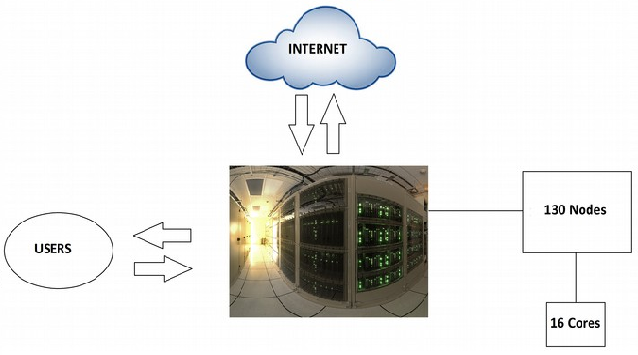
\includegraphics{1.png}
\caption{SuperComputer overview diagram.}
Source: https://commons.wikimedia.org/wiki/File:Wide-angle_view_of_the_ALMA_correlator.jpg
\end{figure}




\section{Product Functions}


\begin{center}

\begin{table}[h!]
\centering
\caption{Project scope table}
\label{my-label}
\begin{tabular}{|l|l|l|}
\hline
\textbf{Event Name                                                                  } & \textbf{Input} \& \textit{output                                                                                                     } & \textbf{Description                                                                                                                                                                                                       } \\ \hline
Starting simulation                                                          & \textit{Computing all current jobs                                                                                          } & \begin{tabular}[c]{@{}l@{}}"Main functionality of supercomputer software;\\ simulation starts creating random users \\ and simulate real life computations adding each \\ user demand (job) to queue"\end{tabular} \\ \hline
\begin{tabular}[c]{@{}l@{}}Setting currnet \\ demand\end{tabular}            & \begin{tabular}[c]{@{}l@{}}\textbf{currentDemandNumber}, \\ \textit{computation resutls}\end{tabular}                                  & \begin{tabular}[c]{@{}l@{}}"Main functionality of user;\\ system's customer will be able to order \\ a job (computation)"\end{tabular}                                                                             \\ \hline
Making users                                                                 & \textit{Users list                                                                                                          } & Creating users for simulation purposes                                                                                                                                                                             \\ \hline
\begin{tabular}[c]{@{}l@{}}Estimating job \\ period\end{tabular}             & \begin{tabular}[c]{@{}l@{}}\textbf{userDemandType}, \\ \textit{Estiamted job time}\end{tabular}                                        & \begin{tabular}[c]{@{}l@{}}Returning estimated time of demanded job \\ selected by user\end{tabular}                                                                                                               \\ \hline
Listing jobs                                                                 & \textit{Job list                                                                                                            } & Users are able to view all jobs in queue                                                                                                                                                                           \\ \hline
\begin{tabular}[c]{@{}l@{}}Providng \\ computation \\ resources\end{tabular} & \begin{tabular}[c]{@{}l@{}}\textbf{Job estimated period}, \\ \textbf{numer of demanded cores},\\\textit{ Number of provided nodes}\end{tabular} & \begin{tabular}[c]{@{}l@{}}Providing resources for each demand, \\ checking if there are available cores and nodes.\end{tabular}                                                                                   \\ \hline
Browsing statistics                                                          & \begin{tabular}[c]{@{}l@{}}\textit{Income, longest job,} \\ \textit{average jobs tim}e\end{tabular}                                    & \begin{tabular}[c]{@{}l@{}}All statistics are showed in a chosen period of \\ time (day/week/month/year)\end{tabular}                                                                                              \\ \hline
\begin{tabular}[c]{@{}l@{}}Managing users \\ balance\end{tabular}            & \textit{Acctual balance                                                                                                     } & \begin{tabular}[c]{@{}l@{}}Notifying each user about their balance; \\ Checking if user balance is high enough \\ for performing selected job\end{tabular}                                                         \\ \hline
Scheduling                                                                   & \textit{Maded Queue                                                                                                         } & \begin{tabular}[c]{@{}l@{}}Making queue using First-come, first-served \\ system\end{tabular}                                                                                                                      \\ \hline
\end{tabular}
\end{table}
\end{center}





\section{Operating Environment}



System was developed for following working environment:
\\
\\
Software:
\begin{itemize}
\item  Windows systems( versions 7/8/10)
\item  Linux Ubuntu Server, Debian
\end{itemize}
 
Hardware:
\begin{itemize}
\item   Athos - iDataPlex DX360M4, Intel Xeon E5-2697v2 12C 2.700GHz, Infiniband FDR14
IBM 	
\item  138 Nodes (including two accelerated nodes and  six specialized nodes,  using for rendering and visualization of complex data)
\item 50 PB of storage
\item 128 GB DDR4 Ram per node
\end{itemize}

\section{Design and Implementation Constraints}



\textbf{Budget:} \pounds 500 000

\textbf{Time:} 2 months
\\
\\
\textbf{Crucial constraints:}
\begin{itemize}
\item   Time constraint 
\item  Performing proper tests. Consider all cases and potential errors places or exceptional situations is unlikely
\item Limited budget
\item Sustaining highest possible performance having reliable system is difficult to implement and to maintain
\item Demand of high C++ knowledge in developer team, it could be hard to get specialist and introduce him to project with constrained time 
\item For enormous jobs there could be lack of operating memory
\item Limited storage gives constraint of less regular backup making
\item Physical machine have to be stored in appropriate conditions, in room with air-conditioning
\end{itemize}
 


\section{User Documentation}

Additionally to this SRS document there are also following sources about supercomputer system:
\begin{itemize}
\item  Code documentation
\item  Document of test plan of software
\end{itemize}


\section{Assumptions and Dependencies}


Third-party tools used for developing process:
\begin{enumerate}
\item  IDE IntelliJ CLion 2016.3
\item  IDE Microfoft Visual Studio 2015 Enterprise
\item  Visual C++ Redistributable for Visual Studio 2015 
\item  Version control system Git 2.11.0
\item  Unit testing library Google Test

\end{enumerate}



\chapter{External Interface Requirements}

\section{User Interfaces}



\begin{table}[h!]
\centering
\caption{User interface requirement - job ordering}
\label{my-label}
\begin{tabular}{|l|l|}
\hline
\multicolumn{2}{|l|}{\textbf{Customer interface requirements}}                                                                                                                                                                   \\ \hline
Requirement \#: 1       & Event/use case \#: Customer - 1,4                                                                                                                                                                      \\ \hline
Description:            & \begin{tabular}[c]{@{}l@{}}System should allow customer to \\ order a job - computation.\end{tabular}                                                                                                  \\ \hline
Rationale:              & \begin{tabular}[c]{@{}l@{}}To provide interface for ordering computation on supercomputer. \\ Interface is can be seen in terminal.\end{tabular}                                                                  \\ \hline
Originator:             & Xxxx Xxxxx - Supercomputer programmer.                                                                                                                                                                 \\ \hline
Fit Criterion:          & \begin{tabular}[c]{@{}l@{}}User can send files to internal supercomputer's \\ storage and order needed high performance \\ computation for given problem.  Interface should be intuitive.\end{tabular} \\ \hline
Priority:               & 9                                                                                                                                                                                                      \\ \hline
Conflicts               & None                                                                                                                                                                                                   \\ \hline
Supporting Materials: - & None                                                                                                                                                                                                   \\ \hline
History:                & Created December 20, 2016                                                                                                                                                                              \\ \hline
\end{tabular}
\end{table}




\begin{table}[h!]
\centering
\caption{User interface requirement - viewing account}
\label{my-label}
\begin{tabular}{|l|l|}
\hline
\multicolumn{2}{|l|}{\textbf{Customer interface requirements}}                                                                                       \\ \hline
Requirement \#: 2     & Event/use case \#: Customer - 1,4                                                                                            \\ \hline
Description:          & \begin{tabular}[c]{@{}l@{}}System should allow customer to look \\ at his job in queue and actual balance\end{tabular}       \\ \hline
Rationale:            & \begin{tabular}[c]{@{}l@{}}To provide interface feature for delivering \\ information about customer's account\end{tabular} \\ \hline
Originator:           & Xxxx Xxxxx - Supercomputer programmer.                                                                                       \\ \hline
Fit Criterion:        & \begin{tabular}[c]{@{}l@{}}User is able to see his current balance \\ and position of his job in queue\end{tabular}          \\ \hline
Priority:             & 9                                                                                                                            \\ \hline
Conflicts             & -                                                                                                                            \\ \hline
Supporting Materials: & -                                                                                                                            \\ \hline
History:              & Created December 20, 2016                                                                                                    \\ \hline
\end{tabular}
\end{table}

\section{Hardware Interfaces}


\begin{table}[h!]
\centering
\caption{Hardware interface requirement}
\label{my-label}
\begin{tabular}{|l|l|}
\hline
\multicolumn{2}{|l|}{\textbf{Hardware interface requirement}}                                                                                                \\ \hline
Requirement \#: 3     & Event/use case \#:  \\ \hline
Description:          & \begin{tabular}[c]{@{}l@{}}Software should works well with given hardware.\\ Should be optimized for it. \\ Low latency communication standard \\InfiniBand is provided\end{tabular}              \\ \hline
Rationale:            & \begin{tabular}[c]{@{}l@{}}To provide high quality supercomputer that usues its \\ hardware efficiently\end{tabular}                  \\ \hline
Originator:           & Xxxx Xxxxx - Hardware specialist.                                                                                                          \\ \hline
Fit Criterion:        & \begin{tabular}[c]{@{}l@{}}Hardware resources are utilized properly by software, \\ computation potential is no wasted\\ Communication in system is fast thanks to\\ InfiniBand system\end{tabular} \\ \hline
Priority:             & 5                                                                                                                                    \\ \hline
Conflicts             & -                                                                                                                                    \\ \hline
Supporting Materials: & -                                                                                                                                    \\ \hline
History:              & Created December 20, 2016                                                                                                            \\ \hline
\end{tabular}
\end{table}

\section{Software Interfaces}
$<$Describe the connections between this product and other specific software 
components (name and version), including databases, operating systems, tools, 
libraries, and integrated commercial components. Identify the data items or 
messages coming into the system and going out and describe the purpose of each.  
Describe the services needed and the nature of communications. Refer to 
documents that describe detailed application programming interface protocols.  
Identify data that will be shared across software components. If the data 
sharing mechanism must be implemented in a specific way (for example, use of a 
global data area in a multitasking operating system), specify this as an 
implementation constraint.$>$

\section{Communications Interfaces}
$<$Describe the requirements associated with any communications functions 
required by this product, including e-mail, web browser, network server 
communications protocols, electronic forms, and so on. Define any pertinent 
message formatting. Identify any communication standards that will be used, such 
as FTP or HTTP. Specify any communication security or encryption issues, data 
transfer rates, and synchronization mechanisms.$>$


\chapter{System Features}


\begin{figure}[h!]
\centering
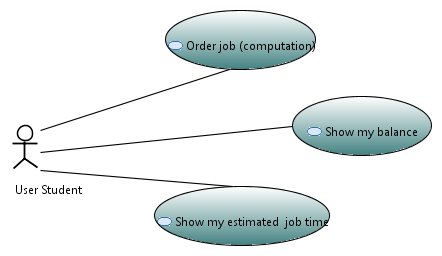
\includegraphics{modelStudent.png}
\caption{User Student use case diagram}
\end{figure}


\begin{figure}[h!]
\centering
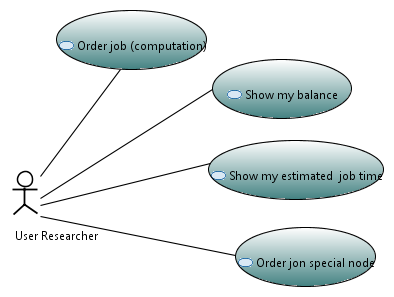
\includegraphics{modelResearcher.png}
\caption{User Researcher use case diagram}
\end{figure}


\begin{figure}[h!]
\centering
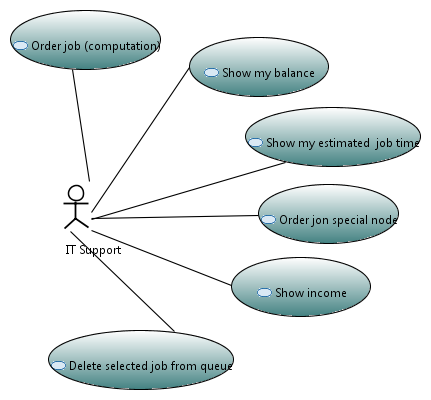
\includegraphics{modelIT.png}
\caption{IT Support use case diagram}
\end{figure}

\section{System Feature - Starting simulation}
$<$Don’t really say “System Feature 1.” State the feature name in just a few 
words.$>$

\subsection{Description and Priority}
$<$Provide a short description of the feature and indicate whether it is of 
High, Medium, or Low priority. You could also include specific priority 
component ratings, such as benefit, penalty, cost, and risk (each rated on a 
relative scale from a low of 1 to a high of 9).$>$

Crucial system feature. Starts whole simulation and shows all job in queue.

\textbf{Priority:} 9



\subsection{Functional Requirements}


\begin{table}[h!]
\centering
\caption{Starting simulation Functional Requirements}
\label{my-label}
\begin{tabular}{|l|l|}
\hline
\multicolumn{2}{|l|}{\textbf{Simulation}}                                                                                                                                                                                                                                                             \\ \hline
Requirement \#: 4     & \begin{tabular}[c]{@{}l@{}}Event/use case \#: Student - 1,2,3; \\ Researcher - 1,2,3,4; \\ IT Support - 1,2,3,4,5\end{tabular}                                                                                                                                                \\ \hline
Description:          & \begin{tabular}[c]{@{}l@{}}Simulation starts creating random users and \\ simulate real life computations adding \\ each user demand (job) to queue\end{tabular}                                                                                                              \\ \hline
Rationale:            & \begin{tabular}[c]{@{}l@{}}To provide simulation output for given\\ number of users\end{tabular}                                                                                                                                                                              \\ \hline
Originator:           & Xxxx Xxxxx - Developers.                                                                                                                                                                                                                                                      \\ \hline
Fit Criterion:        & \begin{tabular}[c]{@{}l@{}}Giving simulation output which uses supercomputer.\\ Output contains all scheduled jobs ordered by users\\ Displaying which user ordered which job, also\\ showing each user balance and estimated time of \\ completion for each job\end{tabular} \\ \hline
Priority:             & 9                                                                                                                                                                                                                                                                             \\ \hline
Conflicts             & -                                                                                                                                                                                                                                                                             \\ \hline
Supporting Materials: & -                                                                                                                                                                                                                                                                             \\ \hline
History:              & Created December 28, 2016                                                                                                                                                                                                                                                     \\ \hline
\end{tabular}
\end{table}



\section{System Feature - Calculating current user's demand }



\subsection{Description and Priority}
This is the most important feature of supercomputer. It gets job defined by user and it perform calculations. System returns output files alter computations. It is important that not each job could be performed each time e.g. user doesn't have enough credits on his account.
\\
\\
\textbf{Feature Priority: } 9

\subsection{Functional Requirements}

\begin{table}[h!]
\centering
\caption{Calculating current user's demand Functional Requirements}
\label{my-label}
\begin{tabular}{|l|l|}
\hline
\multicolumn{2}{|l|}{\textbf{Calculating current demand}}                                                                                                          \\ \hline
Requirement \#: 5     & \begin{tabular}[c]{@{}l@{}}Event/use case \#: \\ Student - 1; \\ Researcher - 1,4; \\ IT Support - 1,4,;\end{tabular}                      \\ \hline
Description:          & Calculating ordered job and returning result output                                                                                        \\ \hline
Rationale:            & Calculating job selected by user                                                                                                           \\ \hline
Originator:           & Xxxx Xxxxx - Developers.                                                                                                                   \\ \hline
Fit Criterion:        & \begin{tabular}[c]{@{}l@{}}Job has to be solved as soon as possible. User will\\ get retult output file afrer job is finished\end{tabular} \\ \hline
Priority:             & 9                                                                                                                                          \\ \hline
Conflicts             & -                                                                                                                                          \\ \hline
Supporting Materials: & -                                                                                                                                          \\ \hline
History:              & Created December 28, 2016                                                                                                                  \\ \hline
\end{tabular}
\end{table}





\section{System Feature - Making users }



\subsection{Description and Priority}
Making random users for simulation purpose. Users type is randomly chosen and rach user job complexity is randomly generated as well.
\\
\\
\textbf{Feature Priority: } 5

\subsection{Functional Requirements}

\begin{table}[]
\centering
\caption{Making users Functional Requirements}
\label{my-label}
\begin{tabular}{|l|l|}
\hline
\multicolumn{2}{|l|}{\textbf{Making users}}                                                                                              \\ \hline
Requirement \#: 6     & Event/use case \#:                                                                                               \\ \hline
Description:          & Making random user for simulation                                                                                \\ \hline
Rationale:            & Returning list of random users                                                                                   \\ \hline
Originator:           & Xxxx Xxxxx - Developers.                                                                                         \\ \hline
Fit Criterion:        & \begin{tabular}[c]{@{}l@{}}Users have to be different and their \\ job need to be different as well\end{tabular} \\ \hline
Priority:             & 5                                                                                                                \\ \hline
Conflicts             & -                                                                                                                \\ \hline
Supporting Materials: & -                                                                                                                \\ \hline
History:              & Created December 28, 2016                                                                                        \\ \hline
\end{tabular}
\end{table}

\section{System Feature - Estimating job period }

\subsection{Description and Priority}
Despite of users choose flag how big (complex) is demand: Small, Medium, Large or Huge supercomputer tries to estimate real computation time in order to manage job queue efficiently.  

\textbf{Feature Priority: } 6

\subsection{Functional Requirements}

\begin{table}[h!]
\centering
\caption{Estimating job period Functional Requirements}
\label{my-label}
\begin{tabular}{|l|l|}
\hline
\multicolumn{2}{|l|}{\textbf{Calculating currnet demand}}                                                                                                   \\ \hline
Requirement \#: 6     & \begin{tabular}[c]{@{}l@{}}Event/use case \#: \\ Student - 1; \\ Researcher - 1,4; \\ IT Support - 1,4,;\end{tabular}               \\ \hline
Description:          & Estimatingj ob period                                                                                                               \\ \hline
Rationale:            & \begin{tabular}[c]{@{}l@{}}Returning\\ estimated time of demanded job selected by user\end{tabular}                                 \\ \hline
Originator:           & Xxxx Xxxxx - Developers.                                                                                                            \\ \hline
Fit Criterion:        & \begin{tabular}[c]{@{}l@{}}System tries to estimate computation period independly\\ of user declration of job duration\end{tabular} \\ \hline
Priority:             & 6                                                                                                                                   \\ \hline
Conflicts             & -                                                                                                                                   \\ \hline
Supporting Materials: & -                                                                                                                                   \\ \hline
History:              & Created December 28, 2016                                                                                                           \\ \hline
\end{tabular}
\end{table}


\section{System Feature - Listing jobs }


\subsection{Description and Priority}

Function that list all current jobs in queue.
\\
\\
\textbf{Feature Priority: } 4

\subsection{Functional Requirements}

\begin{table}[h!]
\centering
\caption{Listing jobs Functional Requirementsn}
\label{my-label}
\begin{tabular}{|l|l|}
\hline
\multicolumn{2}{|l|}{\textbf{Listing jobs}}                                                                                                       \\ \hline
Requirement \#: 7     & \begin{tabular}[c]{@{}l@{}}Event/use case \#: \\ Student - 1; \\ Researcher - 1,4; \\ IT Support - 1,4;\end{tabular}      \\ \hline
Description:          & Listing all jobs in queue                                                                                                 \\ \hline
Rationale:            & Returning list with actual jobs in queue                                                                                  \\ \hline
Originator:           & Xxxx Xxxxx - Developers.                                                                                                  \\ \hline
Fit Criterion:        & \begin{tabular}[c]{@{}l@{}}Return actual job queue in system.\\ Show how much time left to end \\ each job .\end{tabular} \\ \hline
Priority:             & 4                                                                                                                         \\ \hline
Conflicts             & -                                                                                                                         \\ \hline
Supporting Materials: & -                                                                                                                         \\ \hline
History:              & Created December 28, 2016                                                                                                 \\ \hline
\end{tabular}
\end{table}



\section{System Feature - Providing computation resources  }

\subsection{Description and Priority}
Super computer (in spite of it's huge power) as every computer has limitations.
To manage all demands First come, first served  (FCFS) service policy had been used in this supercomputer system. Also there are three types of job size declared by user: Small, Medium, Large, Huge and user can also declare how many cores he needs. This feature assign resources according to job estimated duration. For example for huge jobs computer can grant 4 nodes with 16 cores to use.
\textbf{Feature Priority: } 9

\subsection{Functional Requirements}




\section{System Feature - Browsing statistics  }

\subsection{Description and Priority}

\textbf{Feature Priority: } 9

\subsection{Functional Requirements}




\section{System Feature - Managing users balance   }

\subsection{Description and Priority}

\textbf{Feature Priority: } 9

\subsection{Functional Requirements}



\section{System Feature - Scheduling }

\subsection{Description and Priority}

\textbf{Feature Priority: } 9

\subsection{Functional Requirements}



\chapter{Other Nonfunctional Requirements}

\section{Performance Requirements}
$<$If there are performance requirements for the product under various 
circumstances, state them here and explain their rationale, to help the 
developers understand the intent and make suitable design choices. Specify the 
timing relationships for real time systems. Make such requirements as specific 
as possible. You may need to state performance requirements for individual 
functional requirements or features.$>$

\section{Safety Requirements}
$<$Specify those requirements that are concerned with possible loss, damage, or 
harm that could result from the use of the product. Define any safeguards or 
actions that must be taken, as well as actions that must be prevented. Refer to 
any external policies or regulations that state safety issues that affect the 
product’s design or use. Define any safety certifications that must be 
satisfied.$>$

\section{Security Requirements}
$<$Specify any requirements regarding security or privacy issues surrounding use 
of the product or protection of the data used or created by the product. Define 
any user identity authentication requirements. Refer to any external policies or 
regulations containing security issues that affect the product. Define any 
security or privacy certifications that must be satisfied.$>$

\section{Software Quality Attributes}
$<$Specify any additional quality characteristics for the product that will be 
important to either the customers or the developers. Some to consider are: 
adaptability, availability, correctness, flexibility, interoperability, 
maintainability, portability, reliability, reusability, robustness, testability, 
and usability. Write these to be specific, quantitative, and verifiable when 
possible. At the least, clarify the relative preferences for various attributes, 
such as ease of use over ease of learning.$>$

\section{Business Rules}
$<$List any operating principles about the product, such as which individuals or 
roles can perform which functions under specific circumstances. These are not 
functional requirements in themselves, but they may imply certain functional 
requirements to enforce the rules.$>$


\chapter{Other Requirements}
$<$Define any other requirements not covered elsewhere in the SRS. This might 
include database requirements, internationalization requirements, legal 
requirements, reuse objectives for the project, and so on. Add any new sections 
that are pertinent to the project.$>$

\section{Appendix A: Glossary}
%see https://en.wikibooks.org/wiki/LaTeX/Glossary
$<$Define all the terms necessary to properly interpret the SRS, including 
acronyms and abbreviations. You may wish to build a separate glossary that spans 
multiple projects or the entire organization, and just include terms specific to 
a single project in each SRS.$>$

\section{Appendix B: Analysis Models}
$<$Optionally, include any pertinent analysis models, such as data flow 
diagrams, class diagrams, state-transition diagrams, or entity-relationship 
diagrams.$>$

\section{Appendix C: To Be Determined List}
$<$Collect a numbered list of the TBD (to be determined) references that remain 
in the SRS so they can be tracked to closure.$>$

\end{document}
